\section{Toy decompiler}
\label{toy_decompiler}

\subsection{Introduction}

A modern-day compiler is a product of hundreds of developer/year.
At the same time, toy compiler can be an exercise for a student for a week (or even weekend).

Likewise, commercial decompiler like Hex-Rays can be extremely complex,
while toy decompiler like this one, can be easy to understand and remake.

The following decompiler written in Python, supports only short basic blocks, with no jumps.
Memory is not supported as well.

\subsection{Data structure}

Our toy decompiler will use just one single data structure, representing expression tree.

Many programming textbooks has an example of conversion from Fahrenheit temperature to Celsius, using the following formula:

\begin{center}
{\large $celsius = (fahrenheit - 32) \cdot \frac{5}{9}$}
\end{center}

This expression can be represented as a tree:

% reworked from http://www.texample.net/tikz/examples/decision-tree/
\tikzset{
  treenode/.style = {shape=rectangle, rounded corners,
                     draw, align=center,
                     top color=white, bottom color=blue!20},
  env/.style      = {treenode, font=\ttfamily\normalsize},
}

\begin{center}
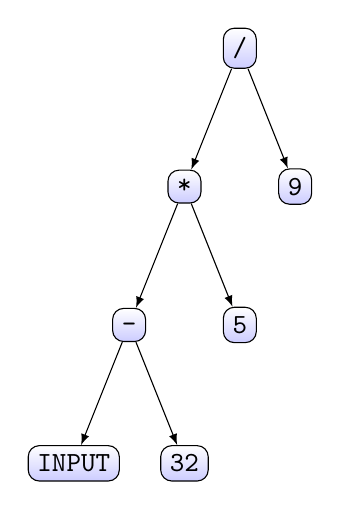
\begin{tikzpicture}
[
	grow                    = down,
	sibling distance        = 4em,
	level distance          = 5em,
	edge from parent/.style = {draw, -latex},
	every node/.style       = {font=\footnotesize},
	sloped
]
\node [env] {/}
	child
	{
		node [env] {*}
		child { 
			node [env] {-}
			child { node [env] {INPUT} }
			child { node [env] {32} }
			}
		child { node [env] {5} }
	}
	child { node [env] {9} }
	;

\end{tikzpicture}
\end{center}


How to store it in memory?
We see here 3 types of nodes: 1) numbers (or values); 2) arithmetical operations; 3) symbols (``INPUT'').

Many developers with \ac{OOP} in their mind will create some kind of class.
Other developer maybe will use ``variant type''.

I'll use simplest possible way of representing this structure: a Python tuple.
First element of tuple can be a string:
either ``EXPR\_OP'' for operations, ``EXPR\_SYMBOL'' for symbol or ``EXPR\_VALUE'' for value.
In case of symbol or value, it follows the string.
In case of operation, the string followed by another tuples.

Node type and operation type is stored as plain string -- to make debugging output easier to read.

There are \textit{constructors} in our code, in \ac{OOP} sense, like these:

\begin{lstlisting}
def create_val_expr (val):
    return ("EXPR_VALUE", val)

def create_symbol_expr (val):
    return ("EXPR_SYMBOL", val)

def create_binary_expr (op, op1, op2):
    return ("EXPR_OP", op, op1, op2)
\end{lstlisting}

There are also \textit{accessors}:

\begin{lstlisting}
def get_expr_type(e):
    return e[0]

def get_symbol (e):
    assert get_expr_type(e)=="EXPR_SYMBOL"
    return e[1]

def get_val (e):
    assert get_expr_type(e)=="EXPR_VALUE"
    return e[1]

def is_expr_op(e):
    return get_expr_type(e)=="EXPR_OP"

def get_op (e):
    assert is_expr_op(e)
    return e[1]

def get_op1 (e):
    assert is_expr_op(e)
    return e[2]

def get_op2 (e):
    assert is_expr_op(e)
    return e[3]
\end{lstlisting}

The conversion expression we just saw will be represented as:

\begin{center}
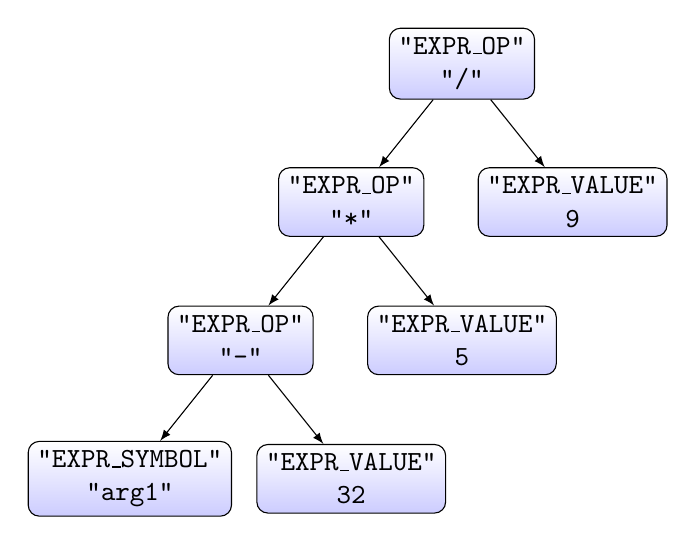
\begin{tikzpicture}
[
	grow                    = down,
	sibling distance        = 8em,
	level distance          = 5em,
	edge from parent/.style = {draw, -latex},
	every node/.style       = {font=\footnotesize},
	sloped
]
\node [env] {"EXPR\_OP"\\"/"}
	child
	{
		node [env] {"EXPR\_OP"\\"*"}
		child { 
			node [env] {"EXPR\_OP"\\"-"}
			child { node [env] {"EXPR\_SYMBOL"\\"arg1"} }
			child { node [env] {"EXPR\_VALUE"\\32} }
			}
		child { node [env] {"EXPR\_VALUE"\\5} }
	}
	child { node [env] {"EXPR\_VALUE"\\9} }
	;

\end{tikzpicture}
\end{center}


... or as Python expression:

\begin{lstlisting}
('EXPR_OP', '/', 
	('EXPR_OP', '*',
	('EXPR_OP', '-', ('EXPR_SYMBOL', 'arg1'), ('EXPR_VALUE', 32)), 
	('EXPR_VALUE', 5)), 
('EXPR_VALUE', 9))
\end{lstlisting}

In fact, this is AST (Abstract Syntax Tree) in its simplest form.
ASTs are heavily used in compilers.

\subsection{Simple examples}

Let's start with simplest example:

\begin{lstlisting}
        mov     rax, rdi
        imul    rax, rsi
\end{lstlisting}

Initial register's values are:
RAX=initial\_RAX,
RBX=initial\_RBX,
RDI=arg1,
RSI=arg2,
RDX=arg3,
RCX=arg4.

When we handle MOV instruction, we just copy expression from RDI to RAX.
When we handle IMUL instruction, we create a new expression, adding together expressions from RAX and RSI and putting
result into RAX again.

I can feed this to decompiler and we will see how register's state is changed through processing:

\begin{lstlisting}
python td.py --show-registers --python-expr tests/mul.s

...

line=[mov       rax, rdi]
rcx=('EXPR_SYMBOL', 'arg4')
rsi=('EXPR_SYMBOL', 'arg2')
rbx=('EXPR_SYMBOL', 'initial_RBX')
rdx=('EXPR_SYMBOL', 'arg3')
rdi=('EXPR_SYMBOL', 'arg1')
rax=('EXPR_SYMBOL', 'arg1')

line=[imul      rax, rsi]
rcx=('EXPR_SYMBOL', 'arg4')
rsi=('EXPR_SYMBOL', 'arg2')
rbx=('EXPR_SYMBOL', 'initial_RBX')
rdx=('EXPR_SYMBOL', 'arg3')
rdi=('EXPR_SYMBOL', 'arg1')
rax=('EXPR_OP', '*', ('EXPR_SYMBOL', 'arg1'), ('EXPR_SYMBOL', 'arg2'))

...

result=('EXPR_OP', '*', ('EXPR_SYMBOL', 'arg1'), ('EXPR_SYMBOL', 'arg2'))
\end{lstlisting}

IMUL instruction is mapped to ``*'' string, and then new expression is constructed in 
handle\_binary\_op(), which puts result into RAX.

In this output, the data structures are dumped using Python str() function, which does mostly the same, as print().

Output is bukly, and we can turn off Python expressions and see how this internal data structure can be rendered neatly
using our internal expr\_to\_string() function:

\begin{lstlisting}
python td.py --show-registers tests/mul.s

...

line=[mov       rax, rdi]
rcx=arg4
rsi=arg2
rbx=initial_RBX
rdx=arg3
rdi=arg1
rax=arg1

line=[imul      rax, rsi]
rcx=arg4
rsi=arg2
rbx=initial_RBX
rdx=arg3
rdi=arg1
rax=(arg1 * arg2)

...

result=(arg1 * arg2)
\end{lstlisting}

Slightly advanced example:

\begin{lstlisting}
        imul    rdi, rsi
        lea     rax, [rdi+rdx]
\end{lstlisting}

LEA instruction is treated just as ADD.

\begin{lstlisting}
python td.py --show-registers --python-expr tests/mul_add.s

...

line=[imul      rdi, rsi]
rcx=('EXPR_SYMBOL', 'arg4')
rsi=('EXPR_SYMBOL', 'arg2')
rbx=('EXPR_SYMBOL', 'initial_RBX')
rdx=('EXPR_SYMBOL', 'arg3')
rdi=('EXPR_OP', '*', ('EXPR_SYMBOL', 'arg1'), ('EXPR_SYMBOL', 'arg2'))
rax=('EXPR_SYMBOL', 'initial_RAX')

line=[lea       rax, [rdi+rdx]]
rcx=('EXPR_SYMBOL', 'arg4')
rsi=('EXPR_SYMBOL', 'arg2')
rbx=('EXPR_SYMBOL', 'initial_RBX')
rdx=('EXPR_SYMBOL', 'arg3')
rdi=('EXPR_OP', '*', ('EXPR_SYMBOL', 'arg1'), ('EXPR_SYMBOL', 'arg2'))
rax=('EXPR_OP', '+', ('EXPR_OP', '*', ('EXPR_SYMBOL', 'arg1'), ('EXPR_SYMBOL', 'arg2')), ('EXPR_SYMBOL', 'arg3'))

...

result=('EXPR_OP', '+', ('EXPR_OP', '*', ('EXPR_SYMBOL', 'arg1'), ('EXPR_SYMBOL', 'arg2')), ('EXPR_SYMBOL', 'arg3'))
\end{lstlisting}

And again, let's see this expression dumped neatly:

\begin{lstlisting}
python td.py --show-registers tests/mul_add.s

...

result=((arg1 * arg2) + arg3)
\end{lstlisting}

Now another example, where we use 2 input arguments:

\begin{lstlisting}
        imul    rdi, rdi, 1234
        imul    rsi, rsi, 5678
        lea     rax, [rdi+rsi]
\end{lstlisting}

\begin{lstlisting}
python td.py --show-registers --python-expr tests/mul_add3.s

...

line=[imul      rdi, rdi, 1234]
rcx=('EXPR_SYMBOL', 'arg4')
rsi=('EXPR_SYMBOL', 'arg2')
rbx=('EXPR_SYMBOL', 'initial_RBX')
rdx=('EXPR_SYMBOL', 'arg3')
rdi=('EXPR_OP', '*', ('EXPR_SYMBOL', 'arg1'), ('EXPR_VALUE', 1234))
rax=('EXPR_SYMBOL', 'initial_RAX')

line=[imul      rsi, rsi, 5678]
rcx=('EXPR_SYMBOL', 'arg4')
rsi=('EXPR_OP', '*', ('EXPR_SYMBOL', 'arg2'), ('EXPR_VALUE', 5678))
rbx=('EXPR_SYMBOL', 'initial_RBX')
rdx=('EXPR_SYMBOL', 'arg3')
rdi=('EXPR_OP', '*', ('EXPR_SYMBOL', 'arg1'), ('EXPR_VALUE', 1234))
rax=('EXPR_SYMBOL', 'initial_RAX')

line=[lea       rax, [rdi+rsi]]
rcx=('EXPR_SYMBOL', 'arg4')
rsi=('EXPR_OP', '*', ('EXPR_SYMBOL', 'arg2'), ('EXPR_VALUE', 5678))
rbx=('EXPR_SYMBOL', 'initial_RBX')
rdx=('EXPR_SYMBOL', 'arg3')
rdi=('EXPR_OP', '*', ('EXPR_SYMBOL', 'arg1'), ('EXPR_VALUE', 1234))
rax=('EXPR_OP', '+', ('EXPR_OP', '*', ('EXPR_SYMBOL', 'arg1'), ('EXPR_VALUE', 1234)), ('EXPR_OP', '*', ('EXPR_SYMBOL', 'arg2'), ('EXPR_VALUE', 5678)))

...

result=('EXPR_OP', '+', ('EXPR_OP', '*', ('EXPR_SYMBOL', 'arg1'), ('EXPR_VALUE', 1234)), ('EXPR_OP', '*', ('EXPR_SYMBOL', 'arg2'), ('EXPR_VALUE', 5678)))
\end{lstlisting}

... and now neat output:

\begin{lstlisting}
python td.py --show-registers tests/mul_add3.s

...

result=((arg1 * 1234) + (arg2 * 5678))
\end{lstlisting}

Now conversion program:

\begin{lstlisting}
        mov     rax, rdi
        sub     rax, 32
        imul    rax, 5
        mov     rbx, 9
        idiv    rbx
\end{lstlisting}

You can see, how register's state is changed over execution (or parsing).

Raw:

\lstinputlisting{toy_decompiler/fahr_raw.txt}

Neat:

\lstinputlisting{toy_decompiler/fahr_neat.txt}

It is interesting to note that IDIV instruction also calculates reminder of division, and it is placed into RDX register.
It's not used, but is ready.

This is how quotient and remainder are stored in registers:

\begin{lstlisting}
def handle_unary_DIV_IDIV (registers, op1):
    op1_expr=register_or_number_in_string_to_expr (registers, op1)
    current_RAX=registers["rax"]
    registers["rax"]=create_binary_expr ("/", current_RAX, op1_expr)
    registers["rdx"]=create_binary_expr ("%", current_RAX, op1_expr)
\end{lstlisting}

Now this is align2grain() function\footnote{Taken from \url{https://docs.oracle.com/javase/specs/jvms/se6/html/Compiling.doc.html}}:

\begin{lstlisting}
        ; uint64_t align2grain (uint64_t i, uint64_t grain)
        ;    return ((i + grain-1) & ~(grain-1));

        ; rdi=i
        ; rsi=grain

        sub     rsi, 1
        add     rdi, rsi
        not     rsi
        and     rdi, rsi
        mov     rax, rdi
\end{lstlisting}

\lstinputlisting{toy_decompiler/align2grain.txt}

\subsection{Dealing with compiler optimizations}

The following piece of code...

\begin{lstlisting}
        mov     rax, rdi
        add     rax, rax
\end{lstlisting}

... will be transormed into \textit{(arg1 + arg1)} expression.
It can be reduced to \textit{(arg1 * 2)}.
Our toy decompiler can indetify such patterns and rewrite them.

\begin{lstlisting}
# X+X -> X*2
def reduce_ADD1 (expr):
    if is_expr_op(expr) and get_op (expr)=="+" and get_op1 (expr)==get_op2 (expr):
        return dbg_print_reduced_expr ("reduce_ADD1", expr, create_binary_expr ("*", get_op1 (expr), create_val_expr (2)))

    return expr # no match
\end{lstlisting}

This function will just test, if the current node has \textit{EXPR\_OP} type,
operation is ``+'' and both children are equal to each other.
By the way, since our data structure is just tuple of tuples, Python can compare them using plain ``=='' operation.
If the testing is finished successfully, current node is then replaced with new expression:
we take one of children, we construct \textit{EXPR\_VALUE} node with ``2'' number in it,
and then we construct \textit{EXPR\_OP} node with ``*'' string as operation.

\textit{dbg\_print\_reduced\_expr()} serving solely debugging purposes --
it just prints the old and the new (reduced) expressions.

Decompiler is then traverse expression tree recursively in \textit{deep-first search} fashion.

\begin{lstlisting}
def reduce_step (e):
    if is_expr_op (e)==False:
        return e # expr isn't EXPR_OP, nothing to reduce (we don't reduce EXPR_SYMBOL and EXPR_VAL)

    if is_unary_op(get_op(e)):
        # recreate expr with reduced operand:
        return reducers(create_unary_expr (get_op(e), reduce_step (get_op1 (e))))
    else:
        # recreate expr with both reduced operands:
        return reducers(create_binary_expr (get_op(e), reduce_step (get_op1 (e)), reduce_step (get_op2 (e))))

...


# same as "return ...(reduce_MUL1 (reduce_ADD1 (reduce_ADD2 (... expr))))"
reducers=compose([
	...
    reduce_ADD1, ...
    ...])

def reduce (e):
    print "going to reduce " + expr_to_string (e)
    new_expr=reduce_step(e)
    if new_expr==e:
        return new_expr # we are done here, expression can't be reduced further
    else:
        return reduce(new_expr) # reduced expr has been changed, so try to reduce it again
\end{lstlisting}

Reduction functions called again and again, as long, as expression changes.

Now we run it:

\begin{lstlisting}
python td.py tests/add1.s

...

going to reduce (arg1 + arg1)
reduction in reduce_ADD1() (arg1 + arg1) -> (arg1 * 2)
going to reduce (arg1 * 2)
result=(arg1 * 2)
\end{lstlisting}

So far so good, now what if we would try this piece of code?

\begin{lstlisting}
        mov     rax, rdi
        add     rax, rax
        add     rax, rax
        add     rax, rax
\end{lstlisting}

\begin{lstlisting}
python td.py tests/add2.s

...

working out tests/add2.s
going to reduce (((arg1 + arg1) + (arg1 + arg1)) + ((arg1 + arg1) + (arg1 + arg1)))
reduction in reduce_ADD1() (arg1 + arg1) -> (arg1 * 2)
reduction in reduce_ADD1() (arg1 + arg1) -> (arg1 * 2)
reduction in reduce_ADD1() ((arg1 * 2) + (arg1 * 2)) -> ((arg1 * 2) * 2)
reduction in reduce_ADD1() (arg1 + arg1) -> (arg1 * 2)
reduction in reduce_ADD1() (arg1 + arg1) -> (arg1 * 2)
reduction in reduce_ADD1() ((arg1 * 2) + (arg1 * 2)) -> ((arg1 * 2) * 2)
reduction in reduce_ADD1() (((arg1 * 2) * 2) + ((arg1 * 2) * 2)) -> (((arg1 * 2) * 2) * 2)
going to reduce (((arg1 * 2) * 2) * 2)
result=(((arg1 * 2) * 2) * 2)
\end{lstlisting}

This is correct, but too verbose.

We would like to rewrite \textit{(X*n)*m} expression to \textit{X*(n*m)}, where $n$ and $m$ are numbers.
We can do this by adding another function like \textit{reduce\_ADD1()}, but there is much better option:
we can make matcher for tree.
You can think about it as regular expression matcher, but over trees.

\begin{lstlisting}
def bind_expr (key):
    return ("EXPR_WILDCARD", key)

def bind_value (key):
    return ("EXPR_WILDCARD_VALUE", key)

def match_EXPR_WILDCARD (expr, pattern):
    return {pattern[1] : expr} # return {key : expr}

def match_EXPR_WILDCARD_VALUE (expr, pattern):
    if get_expr_type (expr)!="EXPR_VALUE":
        return None
    return {pattern[1] : get_val(expr)} # return {key : expr}

def is_commutative (op):
    return op in ["+", "*", "&", "|", "^"]

def match_two_ops (op1_expr, op1_pattern, op2_expr, op2_pattern):
    m1=match (op1_expr, op1_pattern)
    m2=match (op2_expr, op2_pattern)
    if m1==None or m2==None:
        return None # one of match for operands returned False, so we do the same
    # join two dicts from both operands:
    rt={}
    rt.update(m1)
    rt.update(m2)
    return rt

def match_EXPR_OP (expr, pattern):
    if get_expr_type(expr)!=get_expr_type(pattern): # be sure, both EXPR_OP.
        return None
    if get_op (expr)!=get_op (pattern): # be sure, ops type are the same.
        return None

    if (is_unary_op(get_op(expr))):
        # match unary expression.
        return match (get_op1 (expr), get_op1 (pattern))
    else:     
        # match binary expression.     

        # first try match operands as is.
        m=match_two_ops (get_op1 (expr), get_op1 (pattern), get_op2 (expr), get_op2 (pattern))
        if m!=None:
            return m
        # if matching unsuccessful, AND operation is commutative, try also swapped operands.
        if is_commutative (get_op (expr))==False:
            return None
        return match_two_ops (get_op1 (expr), get_op2 (pattern), get_op2 (expr), get_op1 (pattern))

# returns dict in case of success, or None
def match (expr, pattern):
    t=get_expr_type(pattern)
    if t=="EXPR_WILDCARD":
        return match_EXPR_WILDCARD (expr, pattern)
    elif t=="EXPR_WILDCARD_VALUE":
        return match_EXPR_WILDCARD_VALUE (expr, pattern)
    elif t=="EXPR_SYMBOL":
        if expr==pattern:
            return {}
        else:
            return None
    elif t=="EXPR_VALUE":
        if expr==pattern:
            return {}
        else:
            return None
    elif t=="EXPR_OP":
        return match_EXPR_OP (expr, pattern)
    else:
        raise AssertionError
\end{lstlisting}

Now how we will use it:

\begin{lstlisting}
# (X*A)*B -> X*(A*B)
def reduce_MUL1 (expr):
    m=match (expr, create_binary_expr ("*", (create_binary_expr ("*", bind_expr ("X"), bind_value ("A"))), bind_value ("B")))
    if m==None:
        return expr # no match

    return dbg_print_reduced_expr ("reduce_MUL1", expr, create_binary_expr ("*", 
        m["X"], # new op1
        create_val_expr (m["A"] * m["B"]))) # new op2
\end{lstlisting}

We take input expression, and we also construct pattern to be matched.
Matcher works recursively over both expressions synchronously.
Pattern is also expression, but can have two additional node types: \textit{EXPR\_WILDCARD} and
\textit{EXPR\_WILDCARD\_VALUE}. These nodes are supplied by keys (stored as strings).
When matcher encounters \textit{EXPR\_WILDCARD}, it just stashes current expression and will return it.
If matcher encounters \textit{EXPR\_WILDCARD\_VALUE}, matcher do the same, but only in case the current node
has \textit{EXPR\_VALUE} type.

bind\_expr() and bind\_value() functions create nodes with the types we have seen.

All this means, reduce\_MUL1() function will search for the expression in form \textit{(X*A)*B}, where $A$ and $B$
are numbers. In other cases, matcher will return input expression untouched, so these reducing function can be chained.

Now when reduce\_MUL1 encounters (sub)expression we are interesting in, it will return dictionary with keys and expressions.
Let's add \textit{print m} expression somewhere before return and rerun:

\begin{lstlisting}
python td.py tests/add2.s

...

going to reduce (((arg1 + arg1) + (arg1 + arg1)) + ((arg1 + arg1) + (arg1 + arg1)))
reduction in reduce_ADD1() (arg1 + arg1) -> (arg1 * 2)
reduction in reduce_ADD1() (arg1 + arg1) -> (arg1 * 2)
reduction in reduce_ADD1() ((arg1 * 2) + (arg1 * 2)) -> ((arg1 * 2) * 2)
{'A': 2, 'X': ('EXPR_SYMBOL', 'arg1'), 'B': 2}
reduction in reduce_MUL1() ((arg1 * 2) * 2) -> (arg1 * 4)
reduction in reduce_ADD1() (arg1 + arg1) -> (arg1 * 2)
reduction in reduce_ADD1() (arg1 + arg1) -> (arg1 * 2)
reduction in reduce_ADD1() ((arg1 * 2) + (arg1 * 2)) -> ((arg1 * 2) * 2)
{'A': 2, 'X': ('EXPR_SYMBOL', 'arg1'), 'B': 2}
reduction in reduce_MUL1() ((arg1 * 2) * 2) -> (arg1 * 4)
reduction in reduce_ADD1() ((arg1 * 4) + (arg1 * 4)) -> ((arg1 * 4) * 2)
{'A': 4, 'X': ('EXPR_SYMBOL', 'arg1'), 'B': 2}
reduction in reduce_MUL1() ((arg1 * 4) * 2) -> (arg1 * 8)
going to reduce (arg1 * 8)
...
result=(arg1 * 8)
\end{lstlisting}

Dictionary has keys we supplied plus expressions it found.
We then can use them to create new expression and return it.
Numbers are just summed while forming second operand to ``*'' opeartion.

Now a real-world optimization technique --
optimizing GCC replaced multiplication by 31 by shifting and subtraction operations:

\begin{lstlisting}
        mov     rax, rdi
        sal     rax, 5
        sub     rax, rdi
\end{lstlisting}

Without reduction functions, our decompiler will translate this into \textit{((arg1 << 5) - arg1)}.
We can replace shifting left by multiplication:

\begin{lstlisting}
# X<<n -> X*(2^n)
def reduce_SHL1 (expr):
    m=match (expr, create_binary_expr ("<<", bind_expr ("X"), bind_value ("Y")))
    if m==None:
        return expr # no match
    
    return dbg_print_reduced_expr ("reduce_SHL1", expr, create_binary_expr ("*", m["X"], create_val_expr (1<<m["Y"])))
\end{lstlisting}

Now we getting \textit{((arg1 * 32) - arg1)}.
We can add another reduction function:

\begin{lstlisting}
# (X*n)-X -> X*(n-1)
def reduce_SUB3 (expr):
    m=match (expr, create_binary_expr ("-",
        create_binary_expr ("*", bind_expr("X1"), bind_value ("N")),
        bind_expr("X2")))
    
    if m!=None and match (m["X1"], m["X2"])!=None:
        return dbg_print_reduced_expr ("reduce_SUB3", expr, create_binary_expr ("*", m["X1"], create_val_expr (m["N"]-1)))
    else:
        return expr # no match
\end{lstlisting}

Matcher will return two X's, and we must be assured that they are equal.
In fact, in previous versions of this toy decompiler, I did comparison with plain ``=='', and it worked.
But we can reuse match() function for the same purpose, because it will process commutative operations better.
For example, if X1 is ``Q+1'' and X2 is ``1+Q'', expressions are equal, but plain ``=='' will not work.
On the other side, match() function, when encounter ``+'' operation (or another commutative operation),
and it fails with comparison, it will also try swapped operand and recheck again.

However, to understand it easier, for a moment, you can imagine there is ``=='' instead of the second match().

Anyway, here is what we've got:

\begin{lstlisting}
working out tests/mul31_GCC.s
going to reduce ((arg1 << 5) - arg1)
reduction in reduce_SHL1() (arg1 << 5) -> (arg1 * 32)
reduction in reduce_SUB3() ((arg1 * 32) - arg1) -> (arg1 * 31)
going to reduce (arg1 * 31)
...
result=(arg1 * 31)
\end{lstlisting}

Another optimization technique is often seen in ARM thumb code: AND-ing a value with number like 0xFFFFFFF0
is done using shifts:

\begin{lstlisting}
        mov rax, rdi
        shr rax, 4
        shl rax, 4
\end{lstlisting}

This code is quite common in ARM thumb code, because it's a headache to encode 32-bit constants using couple of 16-bit
thumb instructions, while single 16-bit instruction can shift by 4 bits left or right.

Also, the expression \textit{(x>>4)<<4} can be jokingly called as ``twitching operator'':
I've heard the ``-{}-i++'' expression was called like this in russian-speaking social networks, it was some kind of meme
(``operator podergivaniya'').

Anyway, these reduction functions will be used:

\begin{lstlisting}
# X>>n -> X / (2^n)
...
def reduce_SHR2 (expr):
    m=match(expr, create_binary_expr(">>", bind_expr("X"), bind_value("Y")))
    if m==None or m["Y"]>=64:
        return expr # no match

    return dbg_print_reduced_expr ("reduce_SHR2", expr, create_binary_expr ("/", m["X"],
        create_val_expr (1<<m["Y"])))

...

# X<<n -> X*(2^n)
def reduce_SHL1 (expr):
    m=match (expr, create_binary_expr ("<<", bind_expr ("X"), bind_value ("Y")))
    if m==None:
        return expr # no match
    
    return dbg_print_reduced_expr ("reduce_SHL1", expr, create_binary_expr ("*", m["X"], create_val_expr (1<<m["Y"])))

...

# FIXME: slow
# returns True if n=2^x or popcnt(n)=1
def is_2n(n):
    return bin(n).count("1")==1


# AND operation using DIV/MUL or SHL/SHR
# (X / (2^n)) * (2^n) -> X&(~((2^n)-1))
def reduce_MUL2 (expr):
    m=match(expr, create_binary_expr ("*", create_binary_expr ("/", bind_expr("X"), bind_value("N1")), bind_value("N2")))
    if m==None or m["N1"]!=m["N2"] or is_2n(m["N1"])==False: # short-circuit expression
        return expr # no match

    return dbg_print_reduced_expr("reduce_MUL2", expr, create_binary_expr ("&", m["X"],
        create_val_expr(~(m["N1"]-1)&0xffffffffffffffff)))
\end{lstlisting}

Now the result:

\begin{lstlisting}
working out tests/AND_by_shifts2.s
going to reduce ((arg1 >> 4) << 4)
reduction in reduce_SHR2() (arg1 >> 4) -> (arg1 / 16)
reduction in reduce_SHL1() ((arg1 / 16) << 4) -> ((arg1 / 16) * 16)
reduction in reduce_MUL2() ((arg1 / 16) * 16) -> (arg1 & 0xfffffffffffffff0)
going to reduce (arg1 & 0xfffffffffffffff0)
...
result=(arg1 & 0xfffffffffffffff0)
\end{lstlisting}

\subsubsection{Division using multiplication}

Division is often replaced by multiplication for performance reasons.

From school-level mathematics, we can remember that division by 3 can be replaced by multiplication by $\frac{1}{3}$.
In fact, sometimes compilers do so for floating-point arithmetics, for example, FDIV instruction in x86 code
can be replaced by FMUL.
At least MSVC 6.0 will replace division by 3 by multiplication by $0.333333...$ and sometimes it's hard to be sure,
what operation was in original source code.

But when we operate over integer values and CPU registers, we can't use fractions.
However, we can rework fraction:

\begin{center}
{\large $result = \frac{x}{3} = x \cdot \frac{1}{3} = x \cdot \frac{1 \cdot MagicNumber}{3 \cdot MagicNumber}$}
\end{center}

Given the fact that division by $2^n$ is very fast, we now should find that $MagicNumber$, for which the following
equation will be true: $2^n = 3 \cdot MagicNumber$.

This code performing division by 10:

\begin{lstlisting}
        mov     rax, rdi
        movabs  rdx, 0cccccccccccccccdh
        mul     rdx
        shr     rdx, 3
        mov     rax, rdx
\end{lstlisting}

Division by $2^{64}$ is somewhat hidden: lower 64-bit of product in RAX is not used (dropped), only higher 64-bit of
product (in RDX) is used and then shifted by additional 3 bits.

RDX register is set during processing of MUL/IMUL like this:

\begin{lstlisting}
def handle_unary_MUL_IMUL (registers, op1):
    op1_expr=register_or_number_in_string_to_expr (registers, op1)
    result=create_binary_expr ("*", registers["rax"], op1_expr)
    registers["rax"]=result
    registers["rdx"]=create_binary_expr (">>", result, create_val_expr(64))
\end{lstlisting}

In other words, the assembly code we have just seen multiplicates by {\Large $\frac{0cccccccccccccccdh}{2^{64+3}}$},
or divides by {\Large $\frac{2^{64+3}}{0cccccccccccccccdh}$}.
To find divisor we just have to divide numerator by denominator.

\begin{lstlisting}
# n = magic number
# m = shifting coefficient
# return = 1 / (n / 2^m) = 2^m / n
def get_divisor (n, m):
    return (2**float(m))/float(n)

# (X*n)>>m, where m>=64 -> X/...
def reduce_div_by_MUL (expr):
    m=match (expr, create_binary_expr(">>", create_binary_expr ("*", bind_expr("X"), bind_value("N")), bind_value("M")))
    if m==None:
        return expr # no match
    
    divisor=get_divisor(m["N"], m["M"])
    return dbg_print_reduced_expr ("reduce_div_by_MUL", expr, create_binary_expr ("/", m["X"], create_val_expr (int(divisor))))
\end{lstlisting}

This works, but we have a problem: this rule takes \textit{(arg1 * 0xcccccccccccccccd) >> 64} expression first and
finds divisor to be equal to $1.25$.
This is correct: result is shifted by 3 bits after (or divided by 8), and $1.25 \cdot 8 = 10$.
But our toy decompiler doesn't support float numbers.

We can solve this problem in the following way: if divisor has fractional part, we postpone reducing, with a hope,
that two subsequent right shift operations will be reduced into single one before:

\begin{lstlisting}
# (X*n)>>m, where m>=64 -> X/...
def reduce_div_by_MUL (expr):
    m=match (expr, create_binary_expr(">>", create_binary_expr ("*", bind_expr("X"), bind_value("N")), bind_value("M")))
    if m==None:
        return expr # no match
    
    divisor=get_divisor(m["N"], m["M"])
    if math.floor(divisor)==divisor:
        return dbg_print_reduced_expr ("reduce_div_by_MUL", expr, create_binary_expr ("/", m["X"], create_val_expr (int(divisor))))
    else:
        print "reduce_div_by_MUL(): postponing reduction, because divisor=", divisor
        return expr
\end{lstlisting}

That works:

\begin{lstlisting}
working out tests/div_by_mult10_unsigned.s
going to reduce (((arg1 * 0xcccccccccccccccd) >> 64) >> 3)
reduce_div_by_MUL(): postponing reduction, because divisor= 1.25
reduction in reduce_SHR1() (((arg1 * 0xcccccccccccccccd) >> 64) >> 3) -> ((arg1 * 0xcccccccccccccccd) >> 67)
going to reduce ((arg1 * 0xcccccccccccccccd) >> 67)
reduction in reduce_div_by_MUL() ((arg1 * 0xcccccccccccccccd) >> 67) -> (arg1 / 10)
going to reduce (arg1 / 10)
result=(arg1 / 10)
\end{lstlisting}

I don't know if this is best solution. In early version of this decompiler, it processed input expression in two passes:
first pass for everything except division by multiplication, and the second pass for the latter.
I don't know which way is better.
Or maybe we could support float numbers in expressions?

Couple of words about better understanding division by multiplication.
Many people miss ``hidden'' division by $2^{32}$ or $2^{64}$,
when lower 32-bit part (or 64-bit part) of product is not used.
Also, there is misconception that modulo inverse is used here. This is close, but not the same thing.
Extended Euclidean algorithm is usually used to find \textit{magic coefficient}, but in fact,
this algorithm is rather used to solve the equation. You can solve it using any other method.
For example, I used Z3 SMT solver to find \textit{magic coefficient}\footnote{\url{https://yurichev.com/tmp/SAT_SMT_DRAFT.pdf}}.
This is overkill, but I used it as a demonstration.
Anyway, Extended Euclidean algorithm is probably the most efficient way to solve it.
Also, needless to mention, the equation is unsolvable for some divisors, because this is diophantine equation
(i.e., equation allowing result to be only integer), since we work on integer CPU registers, after all.

\subsection{Obfuscation/deobfuscation}

Despite simplicity of our decompiler, we can see how to deobfuscate (or optimize) several simple tricks.

For example, this piece of code does nothing:

\begin{lstlisting}
        mov rax, rdi
        xor rax, 12345678h
        xor rax, 0deadbeefh
        xor rax, 12345678h
        xor rax, 0deadbeefh
\end{lstlisting}

We would need these rules to tame it:

\begin{lstlisting}
# (X^n)^m -> X^(n^m)
def reduce_XOR4 (expr):
    m=match(expr, 
        create_binary_expr("^",
            create_binary_expr ("^", bind_expr("X"), bind_value("N")),
                bind_value("M")))
    
    if m!=None:
        return dbg_print_reduced_expr ("reduce_XOR4", expr, create_binary_expr ("^", m["X"], 
            create_val_expr (m["N"]^m["M"])))
    else:
        return expr # no match

...

# X op 0 -> X, where op is ADD, OR, XOR, SUB
def reduce_op_0 (expr):
    # try each:
    for op in ["+", "|", "^", "-"]:
        m=match(expr, create_binary_expr(op, bind_expr("X"), create_val_expr (0)))
        if m!=None:
            return dbg_print_reduced_expr ("reduce_op_0", expr, m["X"])

    # default:
    return expr # no match
\end{lstlisting}

\begin{lstlisting}
working out tests/t9_obf.s
going to reduce ((((arg1 ^ 0x12345678) ^ 0xdeadbeef) ^ 0x12345678) ^ 0xdeadbeef)
reduction in reduce_XOR4() ((arg1 ^ 0x12345678) ^ 0xdeadbeef) -> (arg1 ^ 0xcc99e897)
reduction in reduce_XOR4() ((arg1 ^ 0xcc99e897) ^ 0x12345678) -> (arg1 ^ 0xdeadbeef)
reduction in reduce_XOR4() ((arg1 ^ 0xdeadbeef) ^ 0xdeadbeef) -> (arg1 ^ 0x0)
going to reduce (arg1 ^ 0x0)
reduction in reduce_op_0() (arg1 ^ 0x0) -> arg1
going to reduce arg1
result=arg1
\end{lstlisting}

This piece of code can be obfuscated (or optimized) as well:

\begin{lstlisting}
; toggle last bit

        mov rax, rdi
        mov rbx, rax
        mov rcx, rbx
        mov rsi, rcx
        xor rsi, 12345678h
        xor rsi, 12345679h
        mov rax, rsi
\end{lstlisting}

\begin{lstlisting}
working out tests/t7_obf.s
going to reduce ((arg1 ^ 0x12345678) ^ 0x12345679)
reduction in reduce_XOR4() ((arg1 ^ 0x12345678) ^ 0x12345679) -> (arg1 ^ 1)
going to reduce (arg1 ^ 1)
result=(arg1 ^ 1)
\end{lstlisting}

I also used \textit{aha!}\footnote{\url{http://www.hackersdelight.org/aha/aha.pdf}} superoptimizer to find weird piece of code which does nothing.

\textit{Aha!} is so called superoptimizer, it tries various piece of codes in brute-force manner, in attempt
to find shortest possible alternative for some mathematical operation.
While sane compiler developers use superoptimizers for this task, I tried it in opposite way, to find oddest
pieces of code for some simple operations, including \textit{do nothing} operation.
In past, I used it to find weird alternative to XOR operation\footnote{\url{https://yurichev.com/tmp/SAT_SMT_DRAFT.pdf}}.)

So here is what \textit{aha!} can find for \textit{do nothing} operation:

\begin{lstlisting}
; do nothing (as found by aha)

        mov rax, rdi
        and rax, rax
        or rax, rax
\end{lstlisting}

\begin{lstlisting}
# X & X -> X
def reduce_AND3 (expr):
    m=match (expr, create_binary_expr ("&", bind_expr ("X1"), bind_expr ("X2")))
    if m!=None and match (m["X1"], m["X2"])!=None:
        return dbg_print_reduced_expr("reduce_AND3", expr, m["X1"])
    else:
        return expr # no match

...

# X | X -> X
def reduce_OR1 (expr):
    m=match (expr, create_binary_expr ("|", bind_expr ("X1"), bind_expr ("X2")))
    if m!=None and match (m["X1"], m["X2"])!=None:
        return dbg_print_reduced_expr("reduce_OR1", expr, m["X1"])
    else:
        return expr # no match
\end{lstlisting}

\begin{lstlisting}
working out tests/t11_obf.s
going to reduce ((arg1 & arg1) | (arg1 & arg1))
reduction in reduce_AND3() (arg1 & arg1) -> arg1
reduction in reduce_AND3() (arg1 & arg1) -> arg1
reduction in reduce_OR1() (arg1 | arg1) -> arg1
going to reduce arg1
result=arg1
\end{lstlisting}

This is weirder:

\begin{lstlisting}
; do nothing (as found by aha)

;Found a 5-operation program:
;   neg   r1,rx
;   neg   r2,rx
;   neg   r3,r1
;   or    r4,rx,2
;   and   r5,r4,r3
;   Expr: ((x | 2) & -(-(x)))

        mov rax, rdi
        neg rax
        neg rax
        or rdi, 2
        and rax, rdi
\end{lstlisting}

Rules added (I used ``NEG'' string to represent negation and to be different from subtraction operation,
which is just minus (``-'')):

\label{AND2}
\begin{lstlisting}
# (op(op X)) -> X, where both ops are NEG or NOT
def reduce_double_NEG_or_NOT (expr):
    # try each:
    for op in ["NEG", "~"]:
        m=match (expr, create_unary_expr (op, create_unary_expr (op, bind_expr("X"))))
        if m!=None:
            return dbg_print_reduced_expr ("reduce_double_NEG_or_NOT", expr, m["X"])

    # default:
    return expr # no match

...

# X & (X | ...) -> X
def reduce_AND2 (expr):
    m=match (expr, create_binary_expr ("&", create_binary_expr ("|", bind_expr ("X1"), bind_expr ("REST")), bind_expr ("X2")))
    if m!=None and match (m["X1"], m["X2"])!=None:
        return dbg_print_reduced_expr("reduce_AND2", expr, m["X1"])
    else:
        return expr # no match
\end{lstlisting}

\begin{lstlisting}
going to reduce ((-(-arg1)) & (arg1 | 2))
reduction in reduce_double_NEG_or_NOT() (-(-arg1)) -> arg1
reduction in reduce_AND2() (arg1 & (arg1 | 2)) -> arg1
going to reduce arg1
result=arg1
\end{lstlisting}

I also forced \textit{aha!} to find piece of code which adds 2 with no addition/subtraction operations allowed:

\begin{lstlisting}
; arg1+2, without add/sub allowed, as found by aha:

;Found a 4-operation program:
;   not   r1,rx
;   neg   r2,r1
;   not   r3,r2
;   neg   r4,r3
;   Expr: -(~(-(~(x))))

        mov     rax, rdi
        not     rax
        neg     rax
        not     rax
        neg     rax
\end{lstlisting}

Rule:

\begin{lstlisting}
# (- (~X)) -> X+1
def reduce_NEG_NOT (expr):
    m=match (expr, create_unary_expr ("NEG", create_unary_expr ("~", bind_expr("X"))))
    if m==None:
        return expr # no match
    
    return dbg_print_reduced_expr ("reduce_NEG_NOT", expr, create_binary_expr ("+", m["X"],create_val_expr(1)))
\end{lstlisting}

\begin{lstlisting}
working out tests/add_by_not_neg.s
going to reduce (-(~(-(~arg1))))
reduction in reduce_NEG_NOT() (-(~arg1)) -> (arg1 + 1)
reduction in reduce_NEG_NOT() (-(~(arg1 + 1))) -> ((arg1 + 1) + 1)
reduction in reduce_ADD3() ((arg1 + 1) + 1) -> (arg1 + 2)
going to reduce (arg1 + 2)
result=(arg1 + 2)
\end{lstlisting}

This is artifact of two's complement system of signed numbers representation.
Same can be done for subtraction (just swap negation and NOT operations).

Now let's add some fake luggage to fahrenheit-to-celsius example:

\begin{lstlisting}
        ; celsius = 5 * (fahr-32) / 9
        ; fake luggage:
        mov     rbx, 12345h
        mov     rax, rdi
        sub     rax, 32
        ; fake luggage:
        add     rbx, rax
        imul    rax, 5
        mov     rbx, 9
        idiv    rbx
        ; fake luggage:
        sub     rdx, rax
\end{lstlisting}

It's not a problem for our decompiler, because this noise is left in RDX register, and not used at all:

\lstinputlisting{toy_decompiler/fahr_to_celsius_obf1.txt}

We can try to pretend we affect result with noise:

\begin{lstlisting}
        ; celsius = 5 * (fahr-32) / 9
        ; fake luggage:
        mov     rbx, 12345h
        mov     rax, rdi
        sub     rax, 32
        ; fake luggage:
        add     rbx, rax
        imul    rax, 5
        mov     rbx, 9
        idiv    rbx
        ; fake luggage:
        sub     rdx, rax
        mov     rcx, rax
        ; OR result with garbage (result of fake luggage):
        or      rcx, rdx
        ; the following instruction shouldn't affect result:
        and     rax, rcx
\end{lstlisting}

... but in fact, it's all reduced by reduce\_AND2() function we already saw (\ref{AND2}):

\begin{lstlisting}
working out tests/fahr_to_celsius_obf2.s
going to reduce ((((arg1 - 32) * 5) / 9) & ((((arg1 - 32) * 5) / 9) | ((((arg1 - 32) * 5) % 9) - (((arg1 - 32) * 5) / 9))))
reduction in reduce_AND2() ((((arg1 - 32) * 5) / 9) & ((((arg1 - 32) * 5) / 9) | ((((arg1 - 32) * 5) % 9) - (((arg1 - 32) * 5)
/ 9)))) -> (((arg1 - 32) * 5) / 9)
going to reduce (((arg1 - 32) * 5) / 9)
result=(((arg1 - 32) * 5) / 9)
\end{lstlisting}

We can see that deobfuscation is in fact the same thing as optimization used in compilers.
We can try this function in GCC:

\begin{lstlisting}
int f(int a)
{
	return -(~a);
};
\end{lstlisting}

Optimizing GCC 5.4 (x86) generates this:

\begin{lstlisting}
f:
        mov     eax, DWORD PTR [esp+4]
        add     eax, 1
        ret
\end{lstlisting}

GCC has its own rewriting rules, some of which are, probably, close to what we use here.

\subsection{Tests}

Despite simplicity of the decompiler, it's still error-prone.
We need to be sure that original expression and reduced one are equivalent to each other.

\subsubsection{Evaluating expressions}

First of all, we would just evaluate (or \textit{run}, or \textit{execute})
expression with random values as arguments, and then compare results.

Evaluator do arithmetical operations when possible, recursively.
When any symbol is encountered, its value (randomly generated before) is taken from a table.

\begin{lstlisting}
un_ops={"NEG":operator.neg,
        "~":operator.invert}

bin_ops={">>":operator.rshift,
        "<<":(lambda x, c: x<<(c&0x3f)), # operator.lshift should be here, but it doesn't handle too big counts
        "&":operator.and_,
        "|":operator.or_,
        "^":operator.xor,
        "+":operator.add,
        "-":operator.sub,
        "*":operator.mul,
        "/":operator.div,
        "%":operator.mod}

def eval_expr(e, symbols):
    t=get_expr_type (e)
    if t=="EXPR_SYMBOL":
        return symbols[get_symbol(e)]
    elif t=="EXPR_VALUE":
        return get_val (e)
    elif t=="EXPR_OP":
        if is_unary_op (get_op (e)):
            return un_ops[get_op(e)](eval_expr(get_op1(e), symbols))
        else:
            return bin_ops[get_op(e)](eval_expr(get_op1(e), symbols), eval_expr(get_op2(e), symbols))
    else:
        raise AssertionError

def do_selftest(old, new):
    for n in range(100):
        symbols={"arg1":random.getrandbits(64), 
                "arg2":random.getrandbits(64), 
                "arg3":random.getrandbits(64), 
                "arg4":random.getrandbits(64)}
        old_result=eval_expr (old, symbols)&0xffffffffffffffff # signed->unsigned
        new_result=eval_expr (new, symbols)&0xffffffffffffffff # signed->unsigned
        if old_result!=new_result:
            print "self-test failed"
            print "initial expression: "+expr_to_string(old)
            print "reduced expression: "+expr_to_string(new)
            print "initial expression result: ", old_result
            print "reduced expression result: ", new_result
            exit(0)
\end{lstlisting}

In fact, this is very close to what LISP \textit{EVAL} function does, or even LISP interpreter.
However, not all symbols are set.
If the code is using initial RAX or RBX (to which symbols ``initial\_RAX'' and ``initial\_RBX'' are assigned,
decompiler will stopped with exception, because no random values assigned to these registers,
and these symbols are absent in \textit{symbols} dictionary.

Using this test, I've suddenly found a bug here (despite simplicity of all these reduction rules).
Well, no-one protected from eye strain.
Nevertheless, it has a serious problem: some bugs can be revealed only if one of arguments is $0$, or $1$, or $-1$.
Maybe there are even more special cases exists.

Mentioned above \textit{aha!} superoptimizer tries at least these values as arguments while testing:
1, 0, -1, 0x80000000, 0x7FFFFFFF, 0x80000001, 0x7FFFFFFE, 0x01234567, 0x89ABCDEF, -2, 2, -3, 3,
-64, 64, -5, -31415.

Still, you cannot be sure.
So here we will try Z3 SMT-solver.

\subsubsection{Using Z3 SMT-solver for testing}

SMT-solver can \textit{prove} that two expressions are equivalent to each other.

For example, with the help of \textit{aha!}, I've found another weird piece of code, which does nothing:

\begin{lstlisting}
; do nothing (obfuscation)

;Found a 5-operation program:
;   neg   r1,rx
;   neg   r2,r1
;   sub   r3,r1,3
;   sub   r4,r3,r1
;   sub   r5,r4,r3
;   Expr: (((-(x) - 3) - -(x)) - (-(x) - 3))

        mov rax, rdi
        neg rax
        mov rbx, rax
        ; rbx=-x
        mov rcx, rbx
        sub rcx, 3
        ; rcx=-x-3
        mov rax, rcx
        sub rax, rbx
        ; rax=(-(x) - 3) - -(x)
        sub rax, rcx
\end{lstlisting}

Using toy decompiler, I've found that this piece is reduced to single \textit{arg1} expression:

\begin{lstlisting}
working out tests/t5_obf.s
going to reduce ((((-arg1) - 3) - (-arg1)) - ((-arg1) - 3))
reduction in reduce_SUB2() ((-arg1) - 3) -> (-(arg1 + 3))
reduction in reduce_SUB5() ((-(arg1 + 3)) - (-arg1)) -> ((-(arg1 + 3)) + arg1)
reduction in reduce_SUB2() ((-arg1) - 3) -> (-(arg1 + 3))
reduction in reduce_ADD_SUB() (((-(arg1 + 3)) + arg1) - (-(arg1 + 3))) -> arg1
going to reduce arg1
result=arg1
\end{lstlisting}

But is it correct?
I've added a function which can output expression(s) to SMT-format, it's as simple as a function which converts
expression to string.

And this is SMT-file to be Z3 solver:

\begin{lstlisting}
(assert
    (forall ((arg1 (_ BitVec 64)) (arg2 (_ BitVec 64)) (arg3 (_ BitVec 64)) (arg4 (_ BitVec 64)))
        (=
            (bvsub (bvsub (bvsub (bvneg arg1) #x0000000000000003) (bvneg arg1)) (bvsub (bvneg arg1) #x0000000000000003))
            arg1
        )
    )
)
(check-sat)
\end{lstlisting}

In plain English terms, what we asking it to be sure, that \textit{forall} four 64-bit arguments, two expressions
are equivalent (second is just \textit{arg1}).

The syntax maybe hard to understand, but in fact, this is very close to LISP, and arithmetical operations
are named ``bvsub'', ``bvadd'', etc, because ``bv'' stands for \textit{bit vector}.

While running, Z3 shows ``sat'', meaning ``satisfiable''.
In other words, Z3 couldn't find counterexample for this expression.

In fact, I can rewrite this expression in the following form: \textit{expr1 != expr2}, and we would ask
Z3 to find at least one set of input arguments, for which expressions are not equal to each other:

\begin{lstlisting}
(declare-const arg1 (_ BitVec 64))
(declare-const arg2 (_ BitVec 64))
(declare-const arg3 (_ BitVec 64))
(declare-const arg4 (_ BitVec 64))

(assert
    (not
        (=
            (bvsub (bvsub (bvsub (bvneg arg1) #x0000000000000003) (bvneg arg1)) (bvsub (bvneg arg1) #x0000000000000003))
            arg1
        )
    )
)
(check-sat)
\end{lstlisting}

Z3 says ``unsat'', meaning, it couldn't find any such counterexample.
In other words, for all possible input arguments, results of these two expressions are always equal to each other.

Nevertheless, Z3 is not omnipotent.
It fails to prove equivalence of the code which performs division by multiplication.
First of all, I extended it so boths results will have size of 128 bit instead of 64:

\begin{lstlisting}
(declare-const x (_ BitVec 64))
    (assert
        (forall ((x (_ BitVec 64)))
            (=
                ((_ zero_extend 64) (bvudiv x (_ bv17 64)))
                (bvlshr (bvmul ((_ zero_extend 64) x) #x0000000000000000f0f0f0f0f0f0f0f1) (_ bv68 128))
            )
        )
    )
(check-sat)
(get-model)
\end{lstlisting}

(\textit{bv17} is just 64-bit number 17, etc.)

Z3 works too long without any answer, and I had to interrupt it.

As Z3 developers mentioned, such expressions are hard for Z3 so far:
\url{https://github.com/Z3Prover/z3/issues/514}.

Still, division by multiplication can be tested using previously described brute-force check.

Some of my other Z3 examples and explanations can be found here: \url{https://yurichev.com/tmp/SAT_SMT_DRAFT.pdf}.

\subsection{My other implementations of toy decompiler}

When I made attempt to write it in C++, of course, node in expression was represented using class.
There is also implementation in pure C\footnote{\url{https://github.com/dennis714/random_notes/tree/master/toy\%20decompiler/C}}, node is represented using structure.

Matchers in both C++ and C versions doesn't return any dictionary, but instead, \textit{bind\_value()}
functions takes pointer to a value which will contain value after successful matching.
\textit{bind\_expr()} takes pointer to a pointer, which will points to the part of expressions, again, in case of success.
I took this idea from LLVM.

Here are two pieces of code from LLVM source code with couple of reducing rules:

\begin{lstlisting}
// (X >> A) << A -> X
  Value *X;
  if (match(Op0, m_Exact(m_Shr(m_Value(X), m_Specific(Op1)))))
    return X;
\end{lstlisting}

( \href{http://llvm.org/docs/doxygen/html/InstructionSimplify_8cpp_source.html}{lib/Analysis/InstructionSimplify.cpp} )

\begin{lstlisting}
// (A | B) | C  and  A | (B | C)                  -> bswap if possible.
  // (A >> B) | (C << D)  and  (A << B) | (B >> C)  -> bswap if possible.
  if (match(Op0, m_Or(m_Value(), m_Value())) ||
      match(Op1, m_Or(m_Value(), m_Value())) ||
      (match(Op0, m_LogicalShift(m_Value(), m_Value())) &&
       match(Op1, m_LogicalShift(m_Value(), m_Value())))) {
    if (Instruction *BSwap = MatchBSwap(I))
      return BSwap;
\end{lstlisting}
( \href{https://github.com/numba/llvm-mirror/blob/master/lib/Transforms/InstCombine/InstCombineAndOrXor.cpp}{lib/Transforms/InstCombine/InstCombineAndOrXor.cpp} )

As you can see, my matcher tries to mimic LLVM.
What I call \textit{reduction} is called \textit{folding} in LLVM.

I have also a blog post about LLVM obfuscator, in which LLVM matcher is mentioned: \url{https://yurichev.com/blog/llvm/}.

Python version of toy decompiler uses strings in place where enumerate data type is used in C version
(like OP\_AND, OP\_MUL, etc) and
symbols used in Racket version\footnote{Racket is Scheme (which is, in turn, LISP dialect) dialect.
\url{https://github.com/dennis714/random_notes/tree/master/toy\%20decompiler/Racket}} (like \textit{'OP\_DIV}, etc).
This may be seen as inefficient, nevertheless, thanks to strings interning, only address of strings are compared in
Python version, not strings as a whole. So strings in Python can be seen as possible replacement for LISP symbols.

\subsubsection{Even simpler toy decompiler}

Knowledge of LISP makes you understand all these things naturally, without significant effort.
But when I had no knowledge of it, but still tried to make a simple toy decompiler, I made it using usual text strings
which holded expressions for each registers (and even memory).

So when MOV instruction copies value from one register to another, we just copy string.
When arithmetical instruction occurred, we do string concatenation:

\begin{lstlisting}
std::string registers[TOTAL];

...

// all 3 arguments are strings
switch (ins, op1, op2)
{
    ...
    case ADD:    registers[op1]="(" + registers[op1] + " + " + registers[op2] + ")";
                 break;
    ...
    case MUL:    registers[op1]="(" + registers[op1] + " / " + registers[op2] + ")";
                 break;
    ...
}
\end{lstlisting}

Now you'll have long expressions for each register, represented as strings.
For reducing them, you can use plain simple regular expression matcher.

For example, for the rule \textit{(X*n)+(X*m) -> X*(n+m)}, you can match (sub)string using the following
regular expression: ``((.*)*(.*))+((.*)*(.*))''
\footnote{This regular expression string hasn't been properly escaped,
for the reason of easier readability and understanding.}.
If the string is matched, you're getting 4 groups (or substrings).
You then just compare 1st and 3rd using string comparison function, then you check if
the 2nd and 4th are numbers, you convert them to numbers, sum them and you make new string, consisting
of 1st group and sum, like this: ``"(" + X + "*" + (int(n) + int(m)) + ")"''.

It was naïve, clumsy, it was source of great embarrassment, but it worked correctly.

\subsection{Difference between toy decompiler and commercial-grade one}

Perhaps, someone, who currently reading this article, may rush into extending my source code.
As an exercise, I would say, that the first step could be support of partial registers: i.e., AL, AX, EAX.
This is tricky, but doable.

Another task may be support of FPU x86 instructions (FPU stack modeling isn't a big deal).

The gap between toy decompiler and decompiler like Hex-Rays is still enormous.
Several tricky problems must be solved, at least these:

\begin{itemize}
\item C data types: arrays, structures, pointers, etc.
This problem is virtually non-existent for JVM (Java, etc) and .NET decompilers, because type information
is present in binary files.

\item Basic blocks, C/C++ statements. Mike Van Emmerik in his thesis
\footnote{\url{https://yurichev.com/mirrors/vanEmmerik_ssa.pdf}} shows how this can be tackled using \ac{SSA} forms
(which are also heavily used in compilers).

\item Memory support, incluing local stack. Keep in mind pointer aliasing problem.
Again, decompilers of JVM and .NET files are simpler here.
\end{itemize}

\subsection{Further reading}

There are several interesting open-source attempts to build decompiler.
Both source code and theses are interesting study.

\begin{itemize}
	\item \textit{decomp} by Jim Reuter\footnote{
			\url{http://www.program-transformation.org/Transform/DecompReadMe},
			\url{http://www.program-transformation.org/Transform/DecompDecompiler}}.

	\item \textit{DCC} by Cristina Cifuentes\footnote{
			\url{http://www.program-transformation.org/Transform/DccDecompiler},
			thesis: \url{https://yurichev.com/mirrors/DCC_decompilation_thesis.pdf}}.

		It is interesting that this decompiler supports only one type (\textit{int}).
		Maybe this is a reason why DCC decompiler produces source code with \textit{.B} extension?
		Read more about B typeless language (C predecessor): \url{https://yurichev.com/blog/typeless/}.

	\item \textit{Boomerang} by Mike Van Emmerik, Trent Waddington et al\footnote{
			\url{http://boomerang.sourceforge.net/},
			\url{http://www.program-transformation.org/Transform/MikeVanEmmerik},
			thesis: \url{https://yurichev.com/mirrors/vanEmmerik_ssa.pdf}}.
\end{itemize}

As I've said, LISP knowledge can help to understand this all much easier.
Here is well-known micro-interpreter of LISP by Peter Norvig, also written in Python:
\url{https://web.archive.org/web/20161116133448/http://www.norvig.com/lispy.html},
\url{https://web.archive.org/web/20160305172301/http://norvig.com/lispy2.html}.

Russian translation: \url{https://habrahabr.ru/post/115206/}.

\subsection{The files}

Python version and tests: URL

There are also C and Racket versions, but outdated.

Keep in mind -- this decompiler is still at toy level, and it was tested only on tiny test files supplied.

